\subsection*{Overview}
The Eclipse Integrated Computational Environment (ICE) has had a great track
record of providing a comprehensive environment for general scientific
computing. Tasks such as model input generation, local and remote simulation
execution, and post-simulation data analysis and visualization are all very well
supported in the application. These tasks take care of the majority of needs
for \emph{using} general scientific computing codes, but what about
\emph{developing} those applications to begin with? Is there any way ICE can be
extended to provide support for the development of science codes?

\begin{figure}[h]

\includegraphics[width=\textwidth]{figures/icemenu.png}
\centering
\caption{The ICE Developer Menu}
\label{fig:devmenu}
\end{figure}

The answer is yes! In 2015 ICE was extended to provide support for scientific
application \emph{development} through a custom, extensible \textbf{Developer} 
top-level menu. This menu is shown in Figure
\ref{fig:devmenu} and provides custom actions that enable efficient scientific
application development for both novice and expert users of a given science
code.

The Developer Menu is completely customizable through Eclipse Extension Points.
Specifically, ICE exposes a new extension point:
\emph{org.eclipse.ice.developer.code}. This extension point provides the means
to specify details about a scientific code: its name, category (Framework,
Nuclear, Other, etc\ldots), and where its repository is hosted, just to name a
few. This point also enables the addition of \emph{commands} that point to some
custom subclass of \emph{org.eclipse.core.commands.AbstractHandler} that
performs some task related to the development of the code.

With these extensions exposed as part of an ICE product execution, ICE
handles all the complexity of picking them up and populating the Developer Menu
dynamically at runtime. This feature is shown in Figure \ref{fig:devcloneice},
with an ICE category for ICE development, and another for scientific frameworks.
This process is exactly how ICE developers work on ICE itself - by pulling down
the ICE binary and leveraging the Developer Menu to clone and build ICE, all
within ICE. ICE also provides these hooks for other scientific codes, like the
Multiphysics Object Oriented Simulation Environment (MOOSE) for general
finite-element simulations. ICE provides a hook for cloning MOOSE and for
forking a templated repository for MOOSE Application development.

\begin{figure}[h]
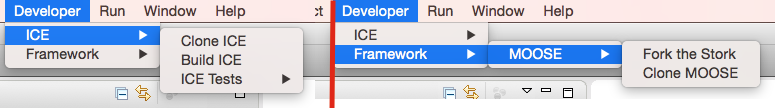
\includegraphics[width=\textwidth]{figures/menu.png}
\caption{The Developer Menu ICE and MOOSE Actions}
\label{fig:devcloneice}
\end{figure}

Extending the Developer Menu is easy, and relies on simply creating a new plugin
and exposing a new extension. Let's see how to do this task in detail:

\subsection*{Extending the ICE Developer Menu}
For this tutorial, we are going to create a hook into the Developer menu to
clone a scientific code called Fern. Fern is an application that provides an
efficient nuclear reaction network solver. It is hosted at
\url{https://github.com/jayjaybillings/fern}. 

To get started, we need to download the ICE plugins to our workspace, which we
can actually do through the Developer menu (pretty cool to use the Developer 
menu to extend the Developer menu!). Click Developer $>$ ICE $>$ Clone ICE to 
get all of ICE's plugins into the workspace. With ICE cloned to the workspace, 
we can now begin to extend the Developer menu. First, we will need to create a
new plugin. 

\subsubsection*{Create a New Plugin Project}
Creating a new plugin for an extension to the ICE Developer menu is simple, just
click File $>$ New $>$ Plugin Project (or Other, then select Plugin Project).
When the wizard opens, name your new plugin with something similar to Figure
\ref{fig:newplugin} and deselect the \texttt{Generate an activatitor} option. On
the next page, simply uncheck the create a plugin from template button and click Finish. 
\begin{figure}[h]
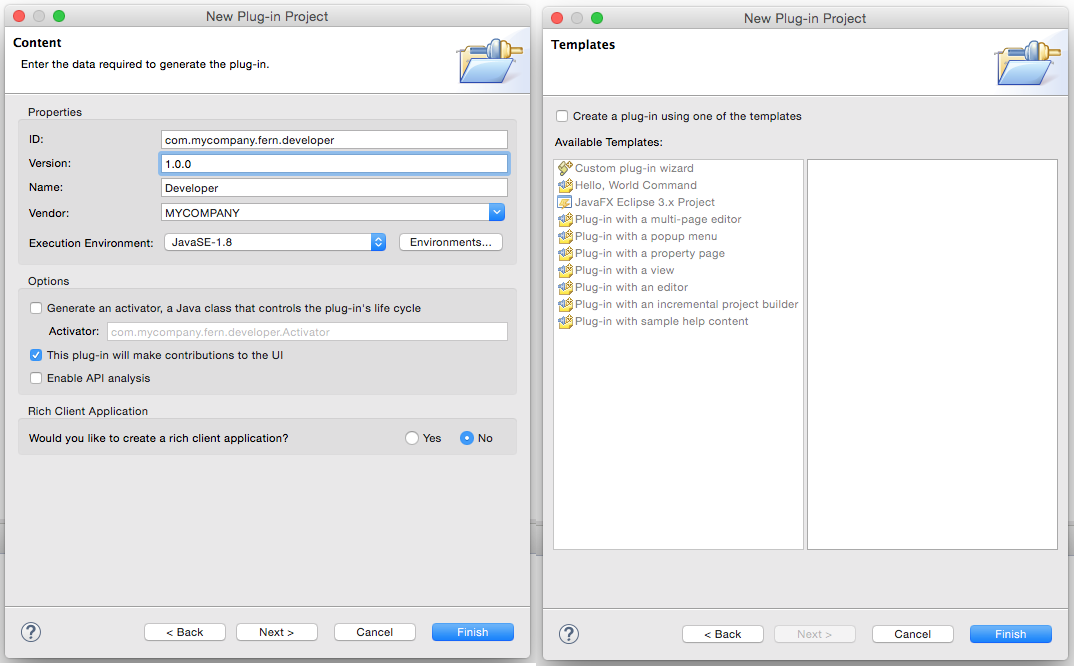
\includegraphics[width=\textwidth]{figures/combinedplugin.png}
\caption{Creating a new Plugin Project}
\label{fig:newplugin}
\end{figure}

When the MANIFEST.MF file editor opens up, add the
\emph{org.eclipse.ice.developer} plugin as a Required Plugin on the Dependencies
tab.

\subsubsection*{Create a New ICE Developer Extension}
Now let's create a new Extension to connect ICE and the Developer Menu
with a Clone Fern action. To do so, go to the Extensions tab of the
plugin MANIFEST file and click add. ICE provides an
org.eclipse.ice.developer.code extension point that lets users define various
details about their codes. 
% \ref{fig:createExtPt} and click Finish.
% \begin{figure}[h]
% 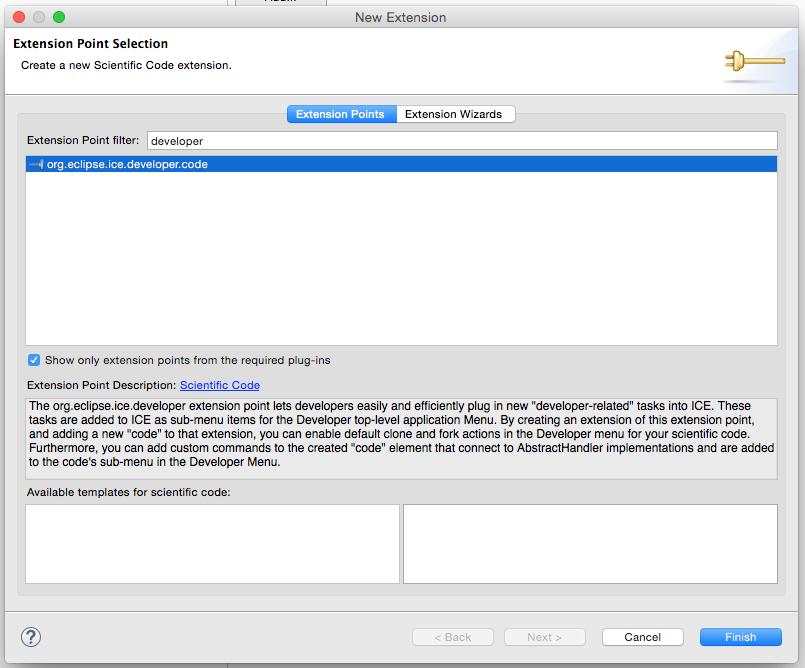
\includegraphics[width=\textwidth]{figures/extensionPt.png}
% \caption{Create a new ICE Scientific Code Extension}
% \label{fig:createExtPt}
% \end{figure}

You will then be presented with the view in Figure \ref{fig:config1}. Enter a
descriptive ID and Name for this extension and click Save. 
\begin{figure}[h]
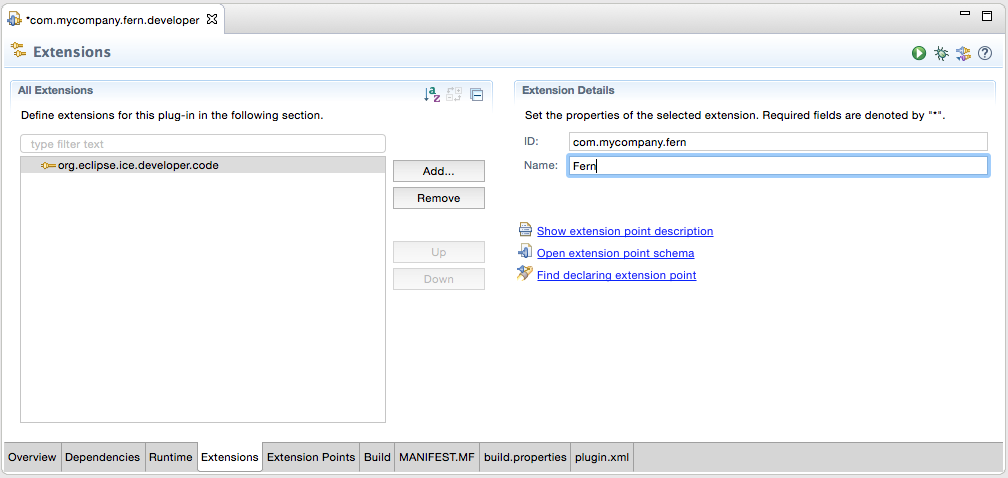
\includegraphics[width=\textwidth]{figures/extptconfig1.png}
\caption{Configure the ID and Name of this Code Extension.}
\label{fig:config1}
\end{figure}

To define your scientific application, right click on the
org.eclipse.ice.developer.code extension in the All Extensions section and
select New $>$ Code in the context menu. This action will present you with the
view in Figure \ref{fig:config2} where you can select the code category, code
display name, the repository URL, and the branch you would like to work with. 

\begin{figure}[h]
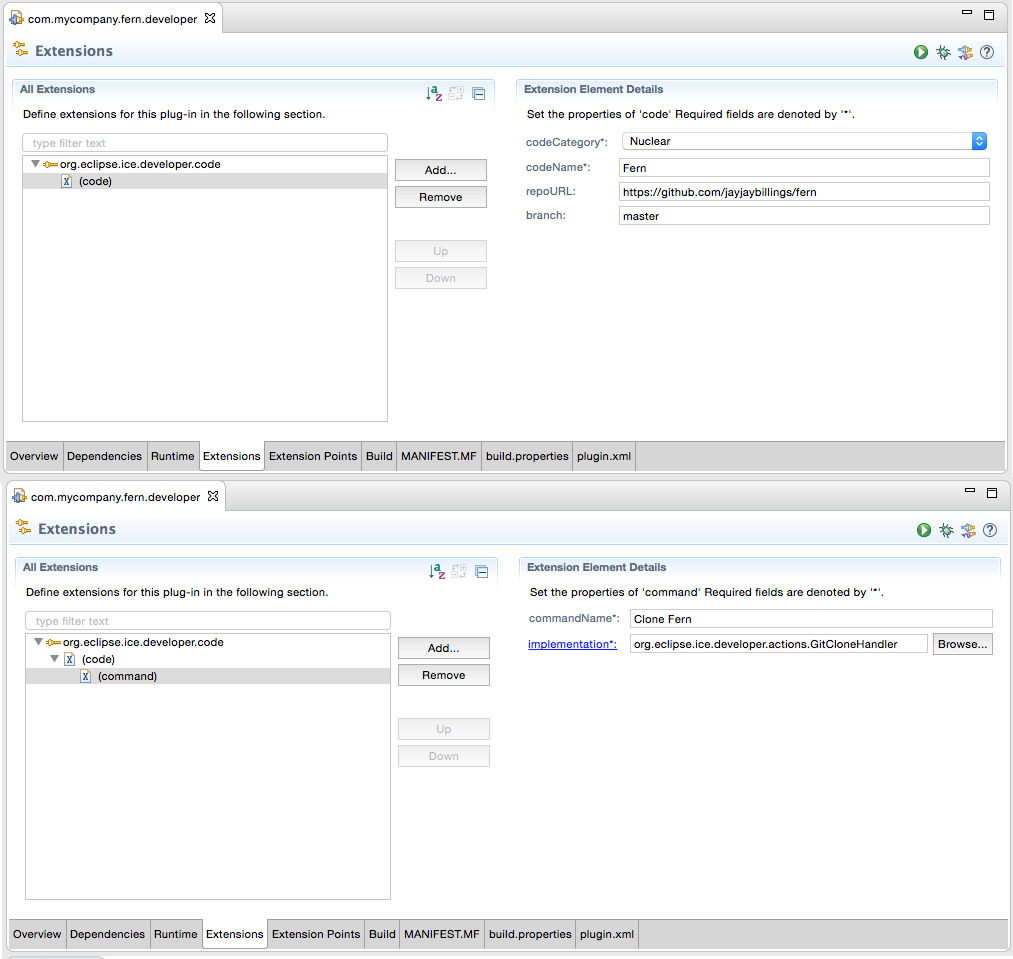
\includegraphics[width=\textwidth]{figures/comb.png}
\caption{Create a new Code description for this extension.}
\label{fig:config2}
\end{figure}

To create a new developer action for your code, right click the code element of
the extension tree and select New $>$ Command. You will then be presented
with the view at the top of Figure \ref{fig:config2} where you can input the
name of this action and the AbstractHandler subclass that performs the action.
ICE provides a default GitCloneHandler that you may select. For this tutorial,
select that and click Save. You should now have a view similar to the bottom of
Figure \ref{fig:config2}.

% \begin{figure}[h]
% 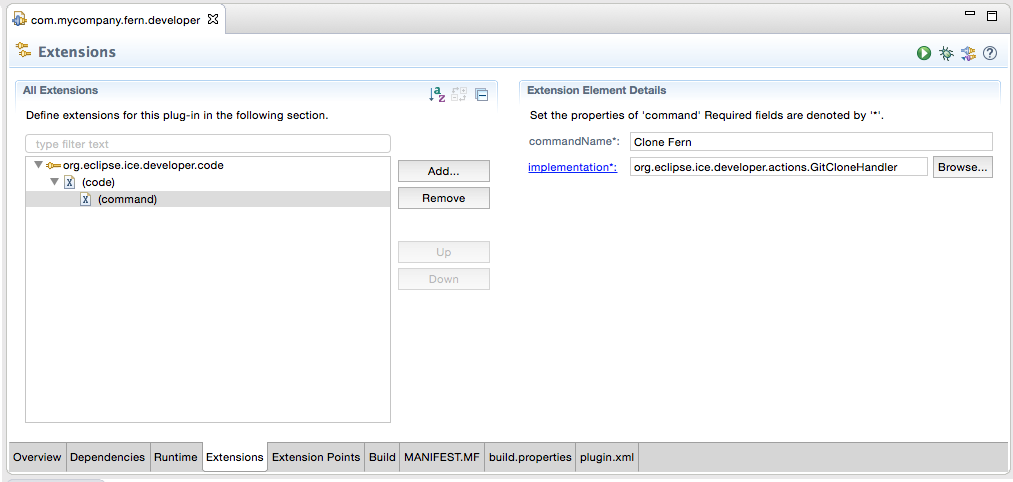
\includegraphics[width=.9\textwidth]{figures/extptconfig4.png}
% \caption{Create a new command for this code extension.}
% \label{fig:config4}
% \end{figure}

\subsubsection*{Setup ICE to Run with the New Plugin}
To see this new Developer command in action, we need to launch a new instance of
ICE. This can be done by opening the Run Configurations Wizard in Run $>$ Run
Configurations. Under the Eclipse Applications element in the tree on the left,
select the ICE launch configuration for your OS. Open the Plugins tab and add
your new developer plugin (see Figure \ref{fig:launch}) by enabling it. Then,
click Run to launch ICE with your developer plugin. 
\begin{figure}[h]
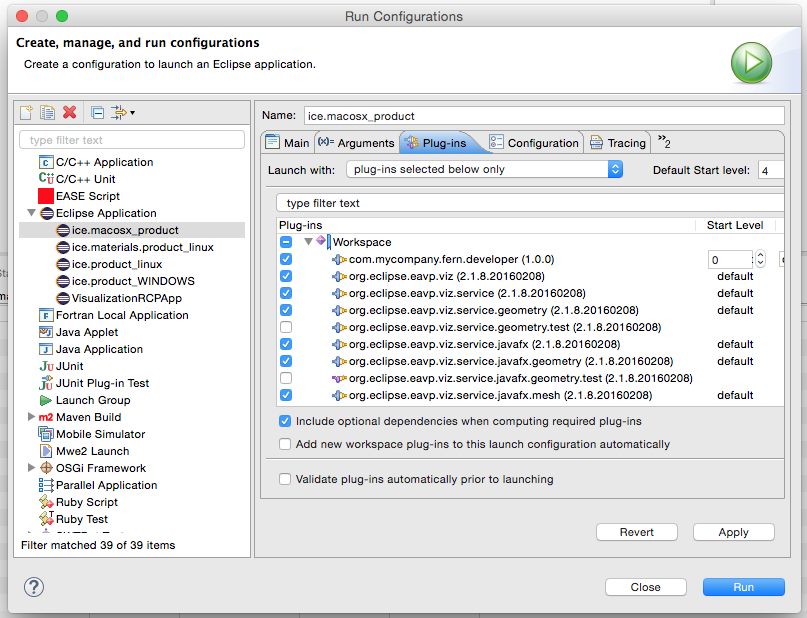
\includegraphics[width=\textwidth]{figures/launch.png}
\caption{Add your plugin to the run configuration.}
\label{fig:launch}
\end{figure}
With ICE running, navigate to the Developer menu and select Nuclear $>$ Fern $>$
Clone Fern (see Figure \ref{fig:clonefern}).
\begin{figure}[h]
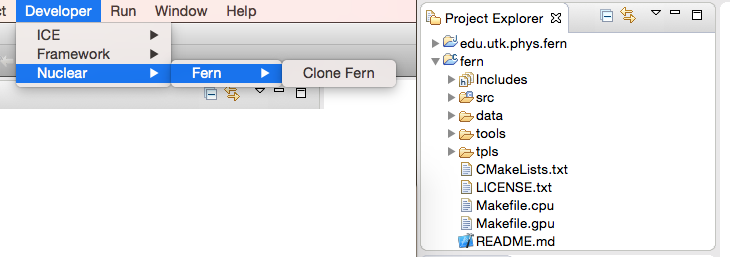
\includegraphics[width=\textwidth]{figures/cloned.png}
\caption{Use the Developer Menu to Clone ICE.}
\label{fig:clonefern}
\end{figure}

This will kick off the action you specified to clone the Fern repository and
pull in any Eclipse projects to the workspace, as shown in Figure
% \ref{fig:result}
% \begin{figure}[h]
% 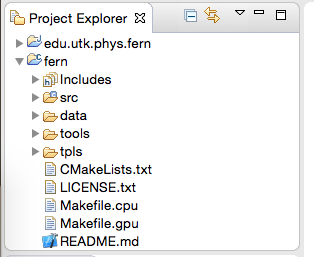
\includegraphics[width=\textwidth]{figures/result.png}
% \label{fig:result}
% \end{figure}